\chapter{系统框架设计}

	本节介绍AppWrapper工具包。与传统的appwrapping技术不同,此工具包可以在字节码级别添加安全功能,以使方法单元上的应用程序不安全,并控制是否通过动态策略管理启用安全功能。如图\ref{fig_1}所示,AppWrapper工具包由三部分组成:自动app包装,实时app流确认和策略设置,以及动态策略管理。
	
	\begin{figure}[hbt]
		\centering
		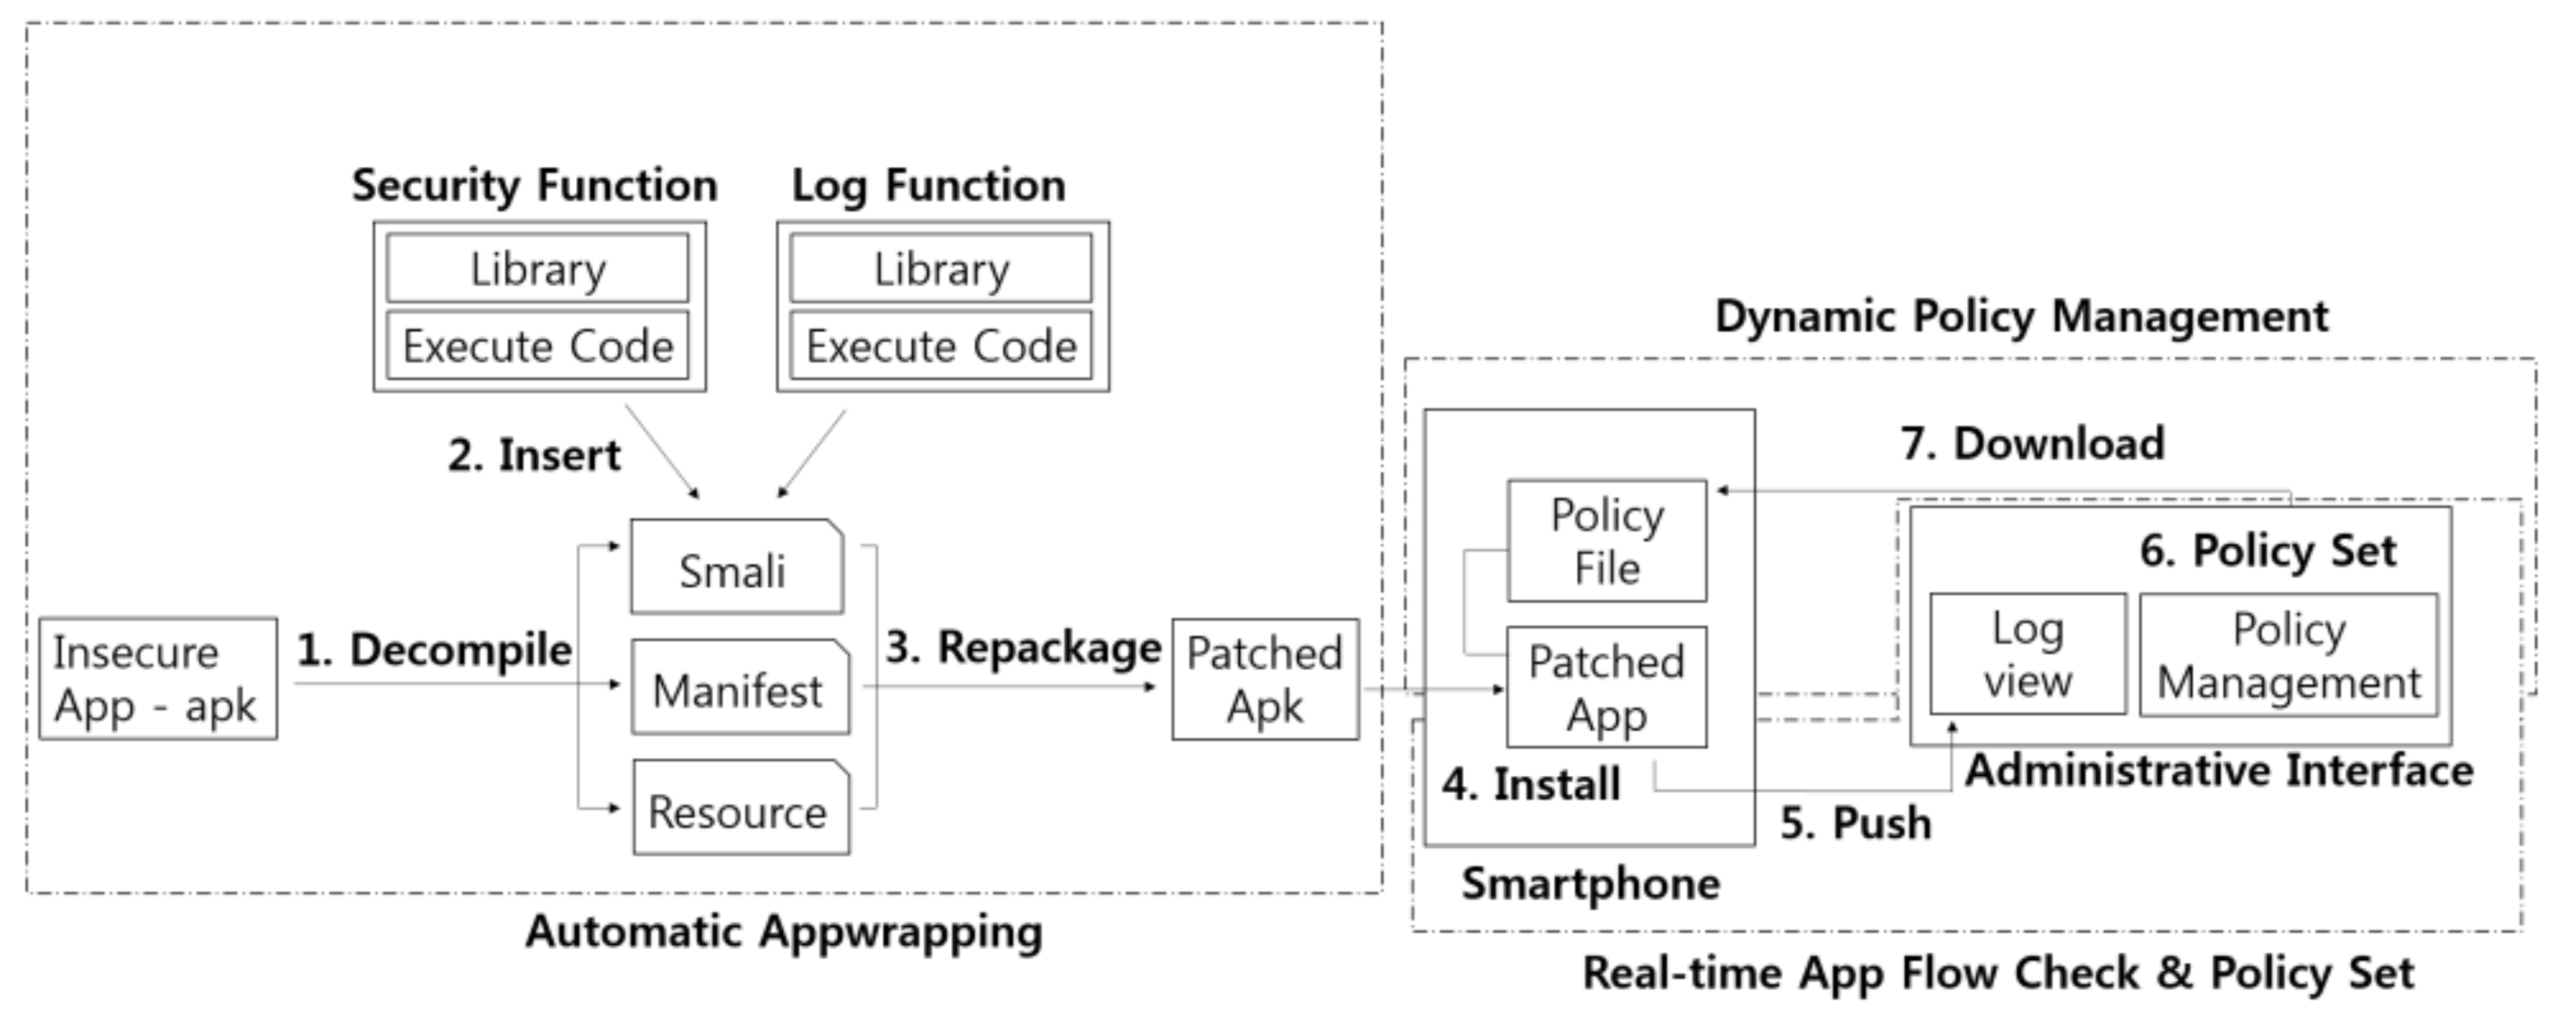
\includegraphics[width=.7\textwidth]{fig1}
		\caption{AppWrapper 概述}
		\label{fig_1}
	\end{figure}

	
	\begin{enumerate}
		\item 反编译不安全应用程序的.apk以获取smali文件作为字节码级别,AndroidManifest.xml文件和资源文件。
		\item 在步骤1中添加在smali code和smali文件中提取的安全性功能和日志应用程序功能。
		\item 使用安全功能和日志功能,现有AndroidManifest.xml文件和资源文件重新打包smali文件,以创建修补的.apk文件。
		\item 在智能手机上安装生成的.apk文件。
		\item 运行已修补的应用程序时,驱动信息(活动类名称,方法名称)将根据应用程序进度的流程发送到AppWrapper工具箱的UI的日志视图。
		\item 检查日志视图并根据应用程序的进度流程将策略设置为在需要安全功能的位置运行安全功能。
		\item 一旦设置了所有必要的安全策略,请将策略文件下载到用户的电话并运行修补的应用程序。修补应用程序的安全功能根据应用程序的进度与下载的策略文件一起执行。
	\end{enumerate}

	该流程在以下小节中详细描述。

	\section{应用程序自动包装}
		安全和日志记录功能是在字节码级别添加的,没有Android的原始源代码。有必要对不安全应用程序的.apk文件进行反编译和重新打包(重新编译和签名)。使用apktool.jar文件执行反编译和重新编译过程。通过重新编译获得的.apk文件使用signapk.jar文件进行签名,并转换为可以安装在用户手机中的.apk文件。签名时需要签名密钥。

		通过反编译.apk获得的smali文件是在字节码级别用smali编写的代码集合,其中添加了安全功能和日志功能。添加的位置是活动中的所有方法单位。它被添加到AndroidManifest.xml文件中声明的所有活动类中的所有方法中。安全和日志函数的smali代码被添加到每个方法的开头,以最小化与现有代码的冲突。在smali中,.method和end方法语法分别表示方法的开始和结束。

		在smali中,寄存器区域根据每个方法中声明的局部变量和输入参数的数量进行分配。在要分配的寄存器区域中有4位,8位和16位,并且对于这些分配中的每一个,指令是不同的。安全性和日志功能代码使用三个局部变量。对于4位寄存器,可以使用从0到15的16个地址编号.Ifa16th addressisusedina4bit寄存器分配方法,发生寄存器错误,重新编译过程失败。为了避免这个问题,通过计算方法中局部变量和参数的数量,将安全性和日志函数添加到仅13个或更少的局部变量分配方法中。这允许添加安全性和日志功能,然后重新打包而不会出现错误。

	\section{动态策略执行}
	
		\begin{figure}[hbt]
			\centering
			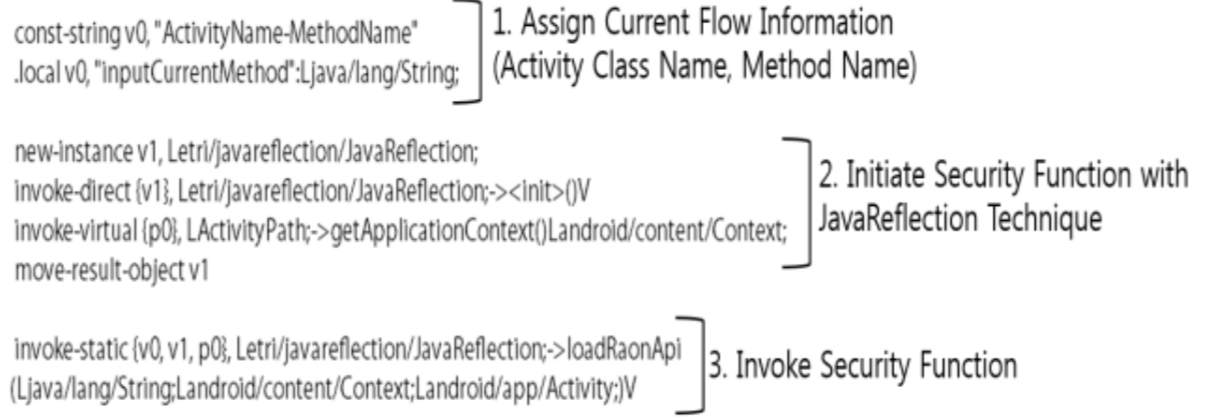
\includegraphics[width=.7\textwidth]{fig2}
			\caption{使用java反射的Smali安全功能代码}
			\label{fig_2}
		\end{figure}

		通过appwrapping添加的安全功能由策略决定。现有的应用程序技术在动态策略管理中存在困难,因为所有与安全相关的代码都包含在基于静态策略添加的安全功能中。但是,建议的AppWrapper可以使用Java反射技术基于动态策略调用和管理各种安全功能。 Java反射技术是一种用于动态加载和使用类的流行技术。通过应用这种技术调用安全函数的smali代码如图\ref{fig_2}所示。当调用安全函数时,它被指定为变量,以便它可以作为参数传输到哪个位置(类名和方法名)叫做。然后,使用Java反射技术初始化安全性函数库,并且与先前分配的变量(类名和方法名)一起调用安全性函数。通过该流程,可以根据app的进度在方法单元中执行安全功能,并且可以灵活地应用各种安全功能。另外,在添加第一个安全功能之后,不需要再次添加安全功能和重新打包过程。由于已将所有安全功能添加到所有方法单元,因此当将新创建的具有已更改策略的策略文件下载到用户的电话时,将自动应用新策略。
				
		可以通过管理界面执行策略设置和管理,如图\ref{fig_3}所示。管理界面由三个单独的屏幕组成:活动类列表和所选活动类和安全功能列表的方法列表。要设置策略,请选择要添加安全功能的活动类,然后选择在活动中执行安全功能的方法位置。然后选择要执行的安全功能。策略设置完成后,将创建策略文件。策略文件包括要执行的安全功能库信息和安全功能信息,以及执行安全功能的位置信息(活动类,方法名称)。表\ref{tab1}显示了一个示例策略文件。安全功能库信息用于使用上述Java反射技术动态调用安全功能。
		
		\begin{table}
			\centering
			\caption{策略文件样本}
			\label{tab1}
			\begin{tabular}{|c|c|c|c|c|}
				\hline
				\# & 活动类 & 方法名 & 安全库 & 安全函数\\
				\hline
				1 & MainActivity & onResume & SecurityApi, SecurityFuntion & FIDO Authentication\\
				\hline
				2 & LoginActivity & onCreate & SecurityApi, SecurityFuntion & Office Model Login\\
				\hline
				3 & LoginActivity & onResume & SecurityApi, SecurityFuntion & Office Model Logout\\
				\hline
			\end{tabular}
		\end{table}

	\section{检查实时应用程序行为并设置策略}
	
		将安全功能添加到不安全的应用程序时,将检查应用程序的进度。 为此,添加了一个日志功能以查看实时应用程序行为。 日志功能使用SSL连接到AppWrapper工具包,并根据应用程序进度流传输日志信息。 通过appwrapping将日志功能添加到修补的应用程序中。 启动修补应用程序后,您可以根据应用程序的流程检查日志信息(类名,方法名称),如图\ref{fig_4}所示。如果单击要设置策略的位置的日志, 您将切换到图\ref{fig_5}的策略设置用户界面屏幕。如果设置策略,则根据应用程序进度流程将安全功能添加到缺乏安全性的位置。
		
		\begin{figure}[hbt]
			\centering
			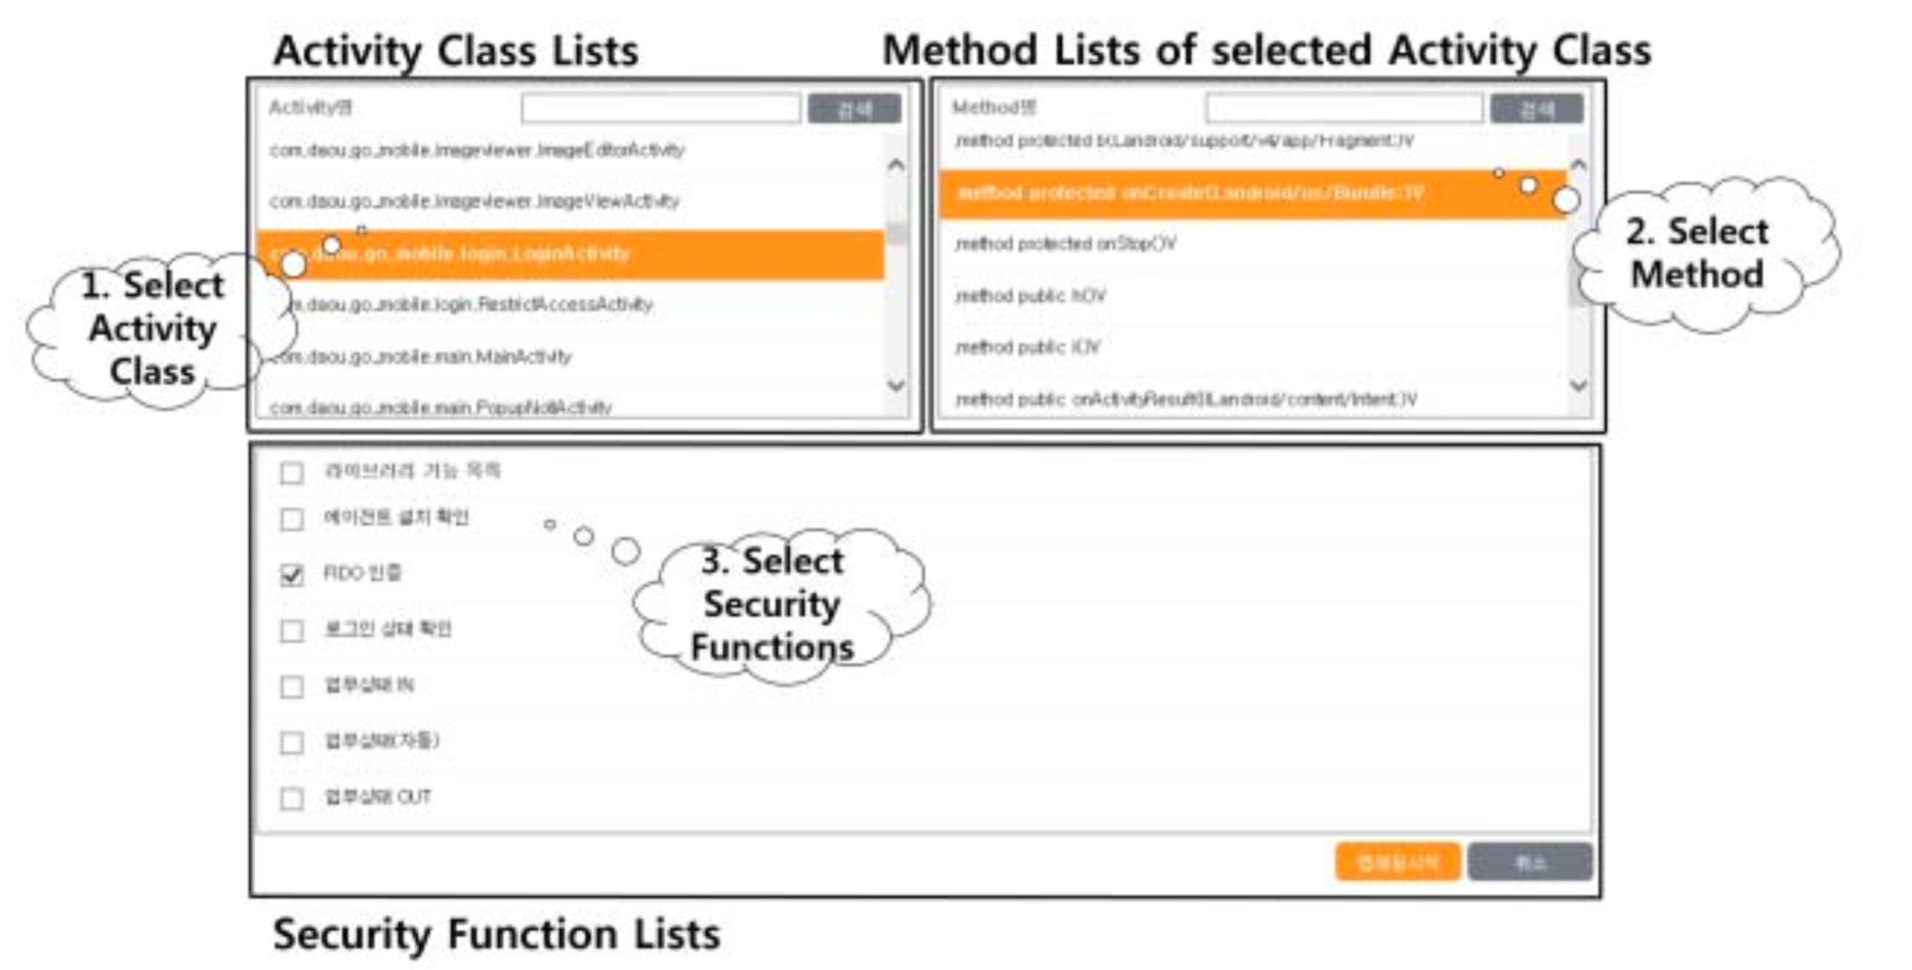
\includegraphics[width=.7\textwidth]{fig3}
			\caption{动态策略管理界面}
			\label{fig_3}
		\end{figure}
		
		\begin{figure}[hbt]
			\centering
			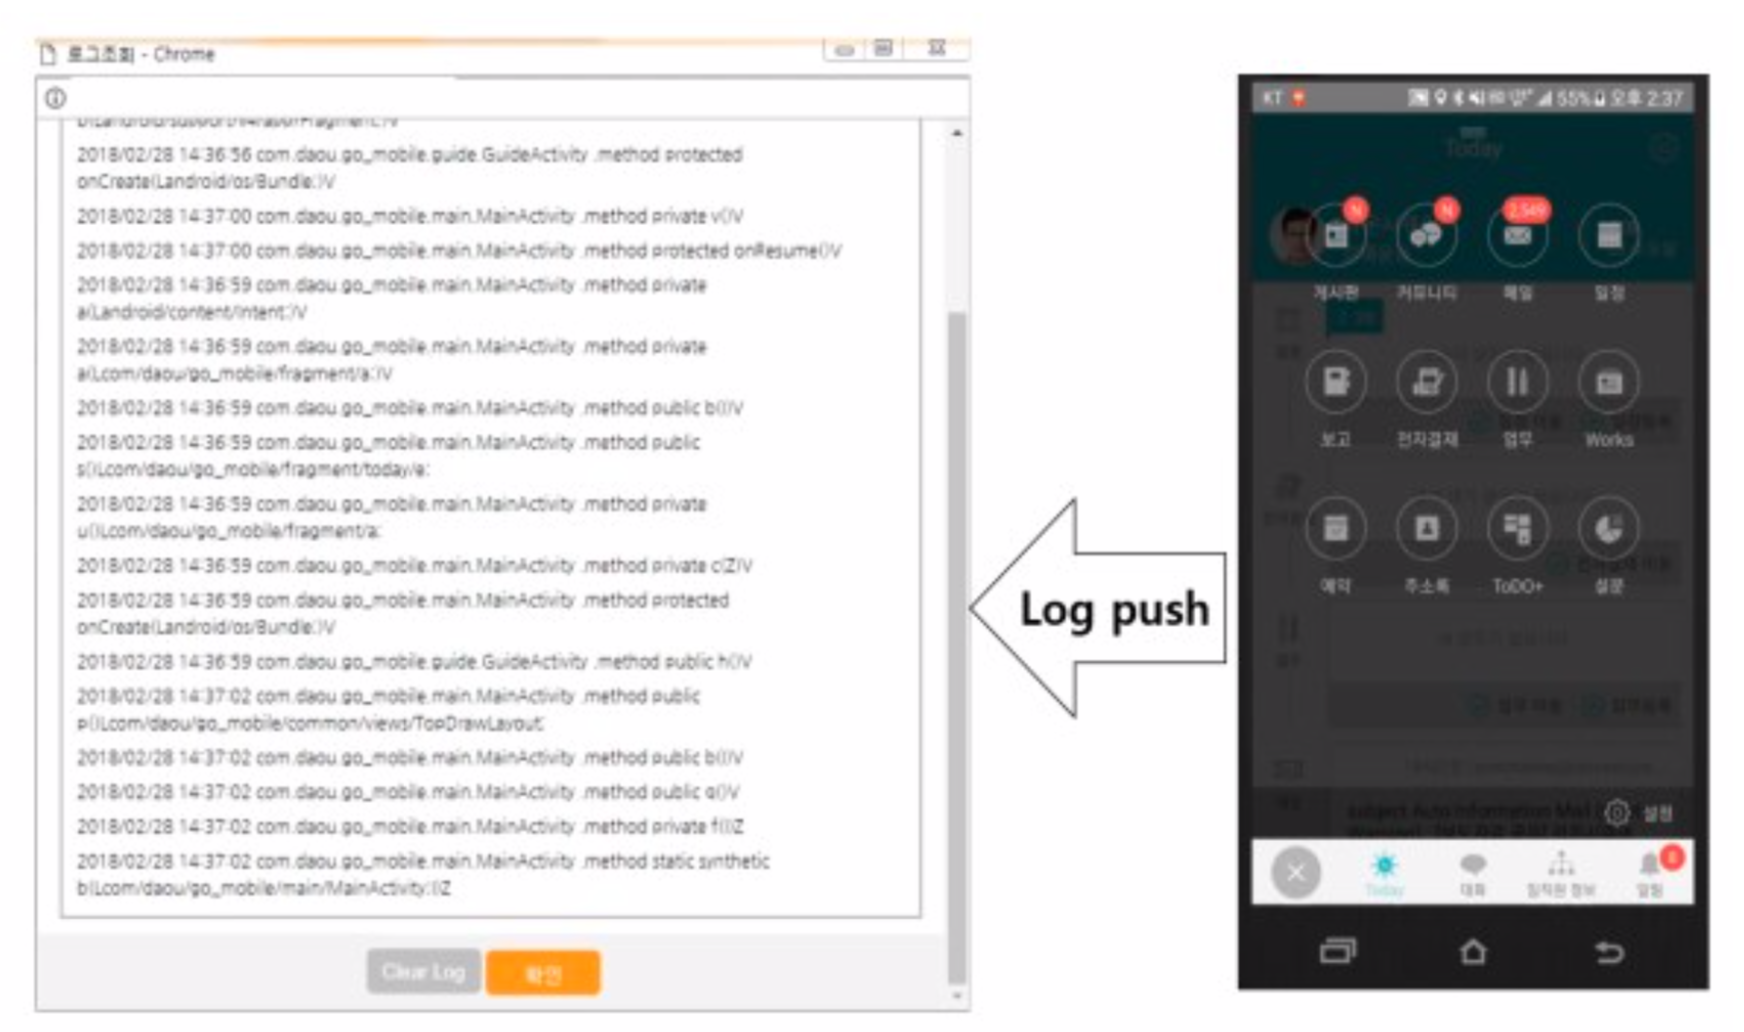
\includegraphics[width=.7\textwidth]{fig4}
			\caption{实时日志视图管理界面}
			\label{fig_4}
		\end{figure}
		
		\begin{figure}[hbt]
			\centering
			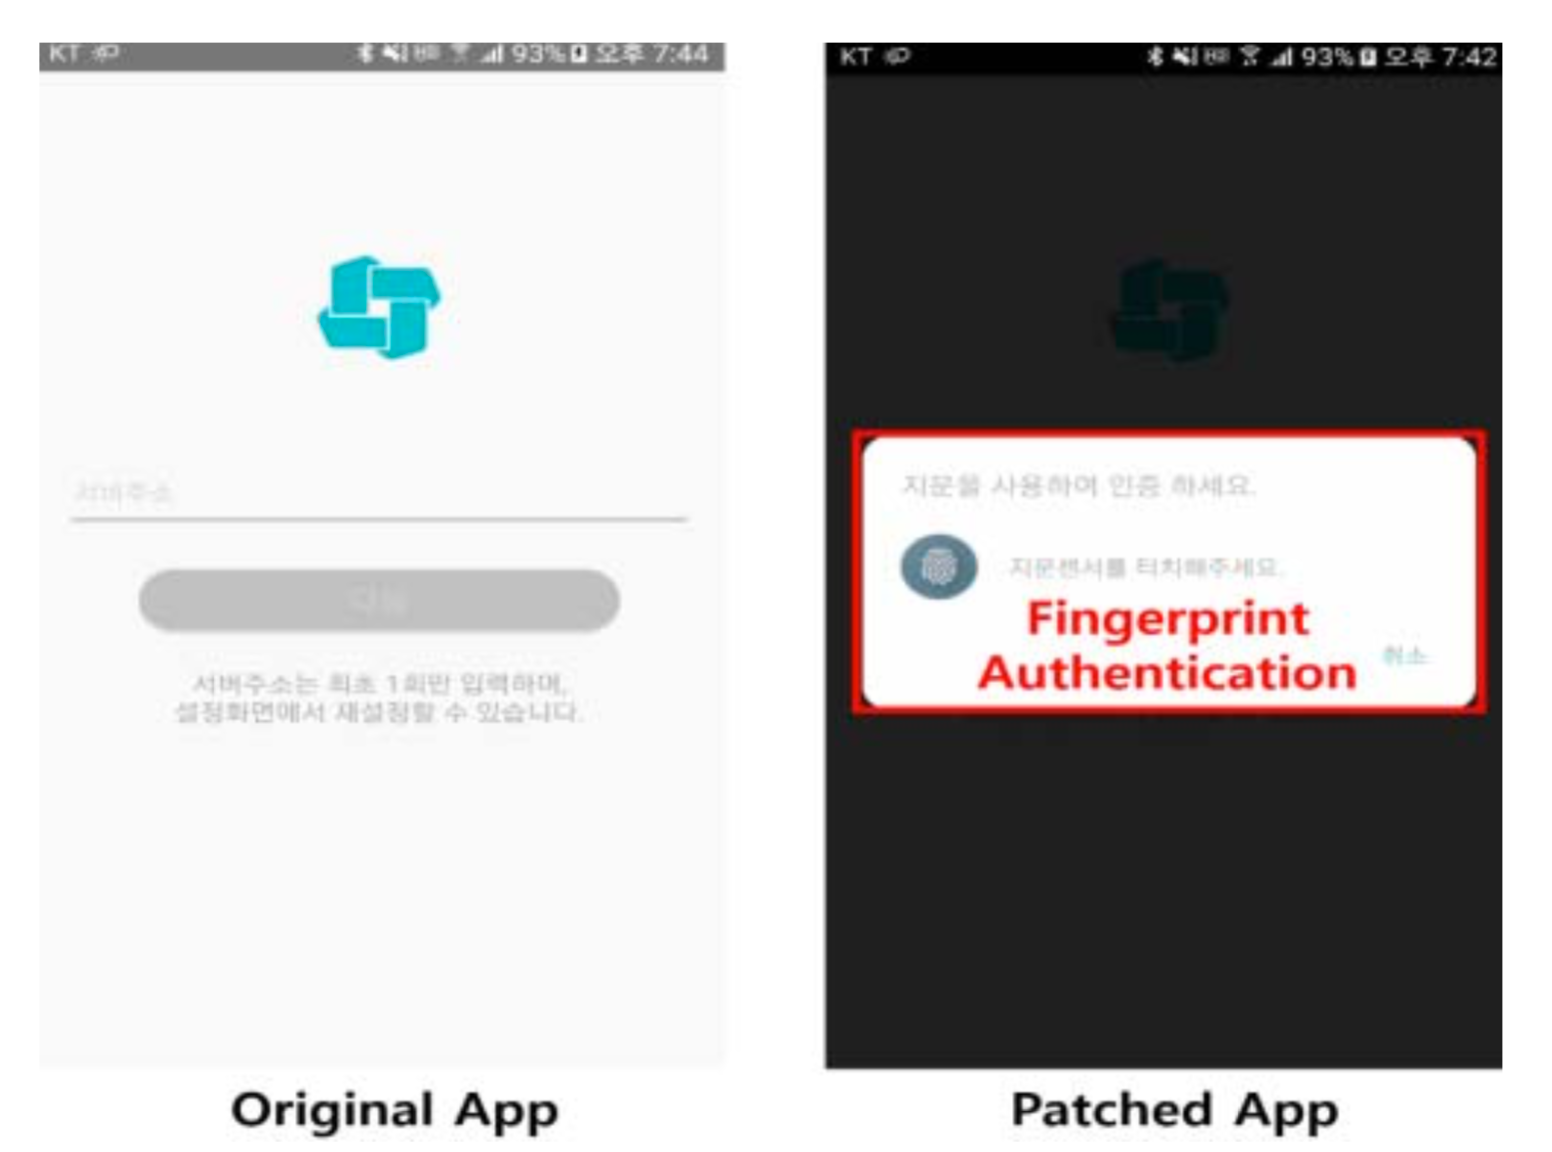
\includegraphics[width=.7\textwidth]{fig5}
			\caption{安全功能补丁前/后的应用启动屏幕}
			\label{fig_5}
		\end{figure}